\documentclass{article}
\usepackage{amsmath}
\usepackage{amssymb}
\usepackage{graphicx}
\usepackage{hyperref}
\usepackage[version=4]{mhchem}

\title{Problem 18}
\date{}

\begin{document}
\maketitle

\section*{Problem}
Prove the Menelaus' Theorem: A line intersects the sides or extension of the sides \(A B, B C\) and \(C A\) of \(\triangle A B C\) at \(X, Y\) and \(Z\), respectively. The following holds \(\frac{A X}{B X} \cdot \frac{B Y}{C Y} \cdot \frac{C Z}{A Z}=1\).\\
\centering
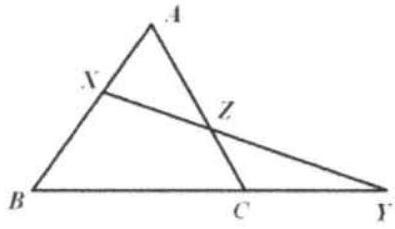
\includegraphics[width=\textwidth]{images/091.jpg}

\section*{Solution}
Solution not available.

\end{document}
